\begin{figure}[h] 
    \centering
    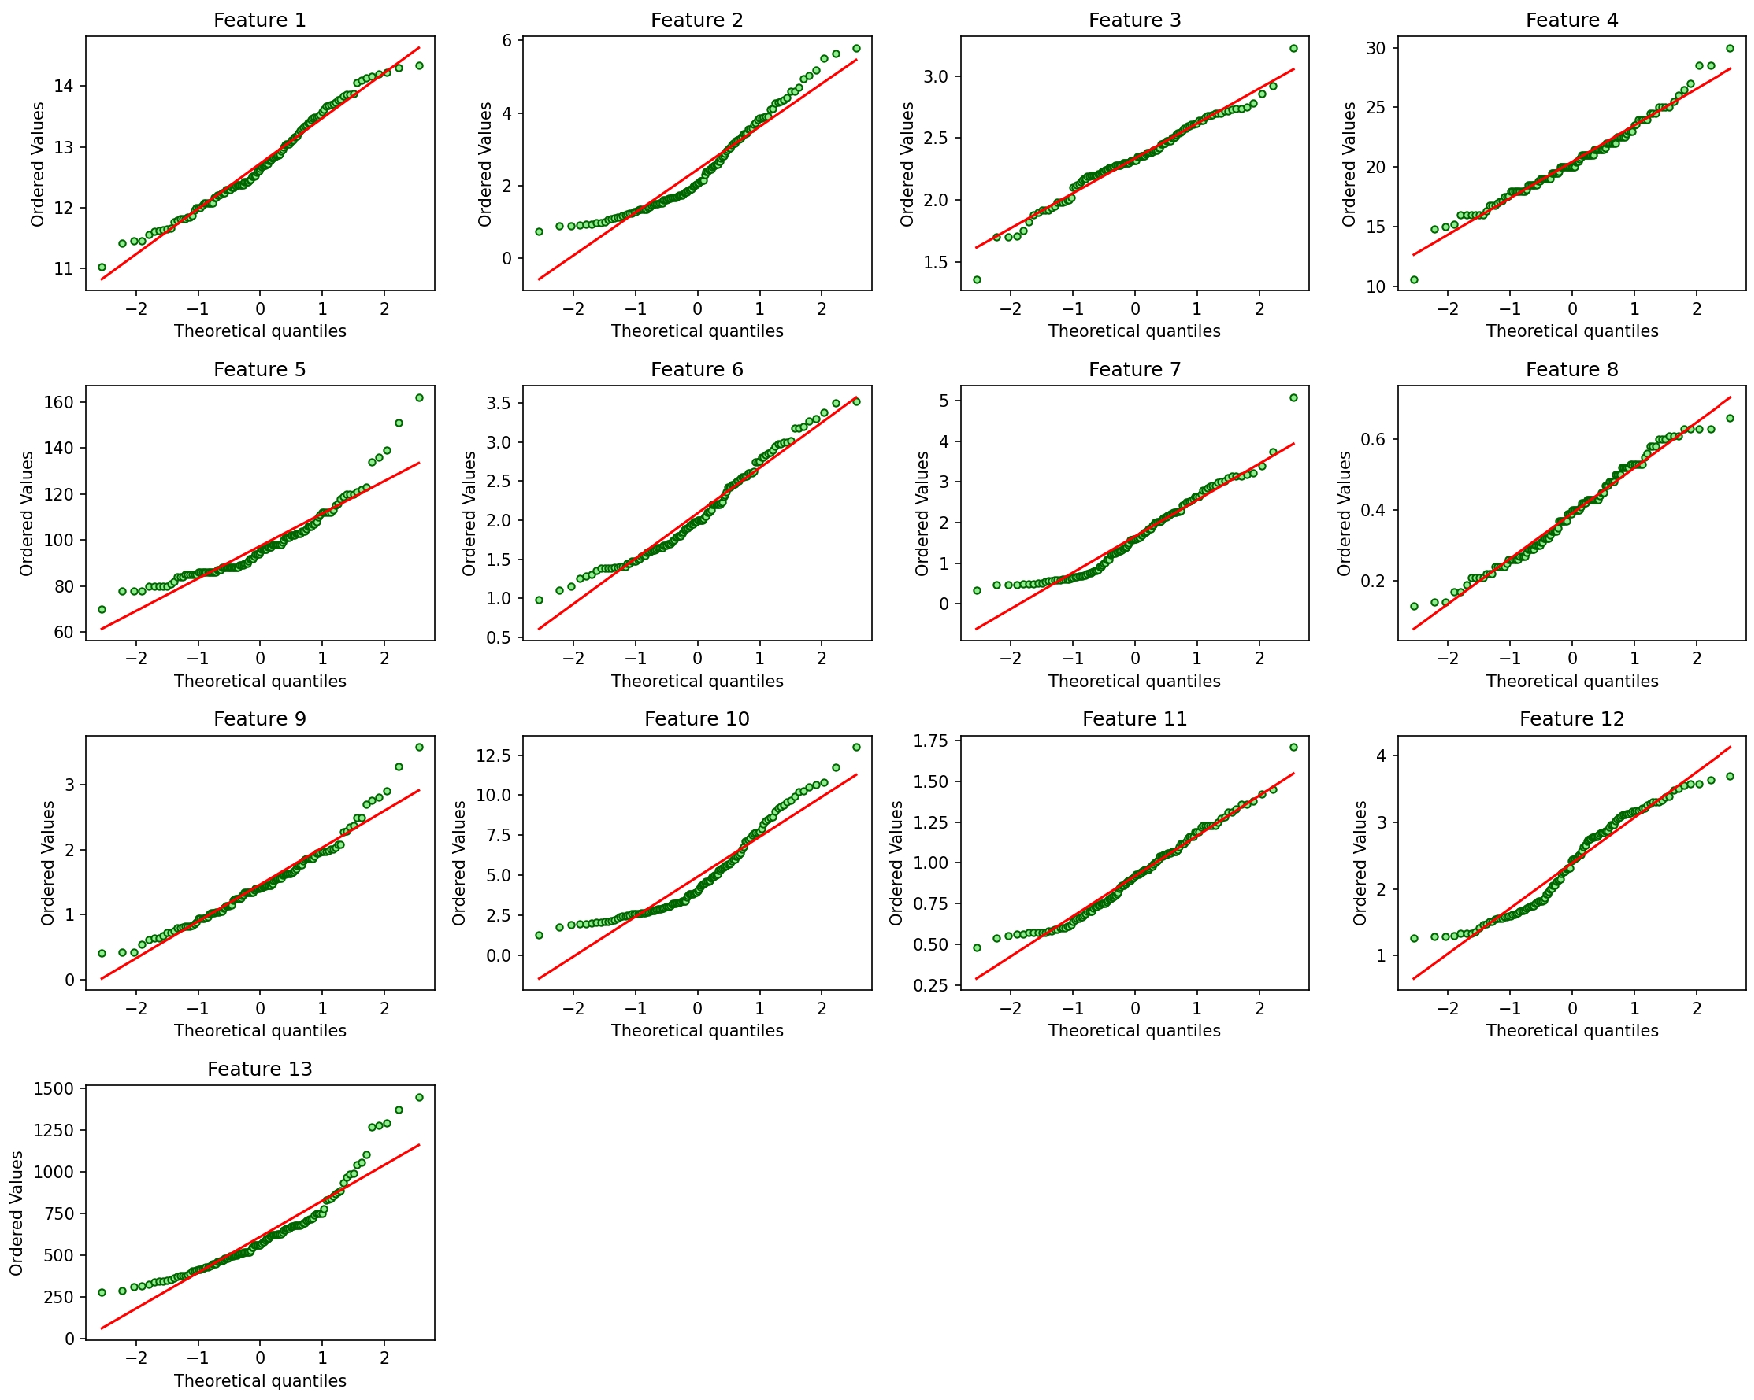
\includegraphics[width=1\textwidth]{Images/Q-Q Plot.pdf}
    \caption{Q-Q Plot.}
    \label{fig:qqpot}
\end{figure}

\begin{table}[h]
\centering
\caption{Results of Shapiro-Wilk test}
\label{tab:shapiro wilk}
\begin{tabular}{lcccccc} 
\toprule
\textbf{Method}         & Statistic & p-value           \\
\midrule
Feature 1               &0.98       &4.22               \\
Feature 2               &0.92       &0.00               \\
Feature 3               &0.98       &\textbf{7.98}      \\
Feature 4               &0.98       &\textbf{10.08}     \\
Feature 5               &0.89       &0.00               \\
Feature 6               &0.96       &0.13               \\
Feature 7               &0.94       &0.00               \\
Feature 8               &0.97       &4.20               \\
Feature 9               &0.95       &0.06               \\
Feature 10              &0.90       &0.00               \\
Feature 11              &0.97       &0.85               \\
Feature 12              &0.94       &0.00               \\
Feature 13              &0.89       &0.00               \\
\bottomrule
\end{tabular}
\end{table}


\begin{figure}[h] 
    \centering
    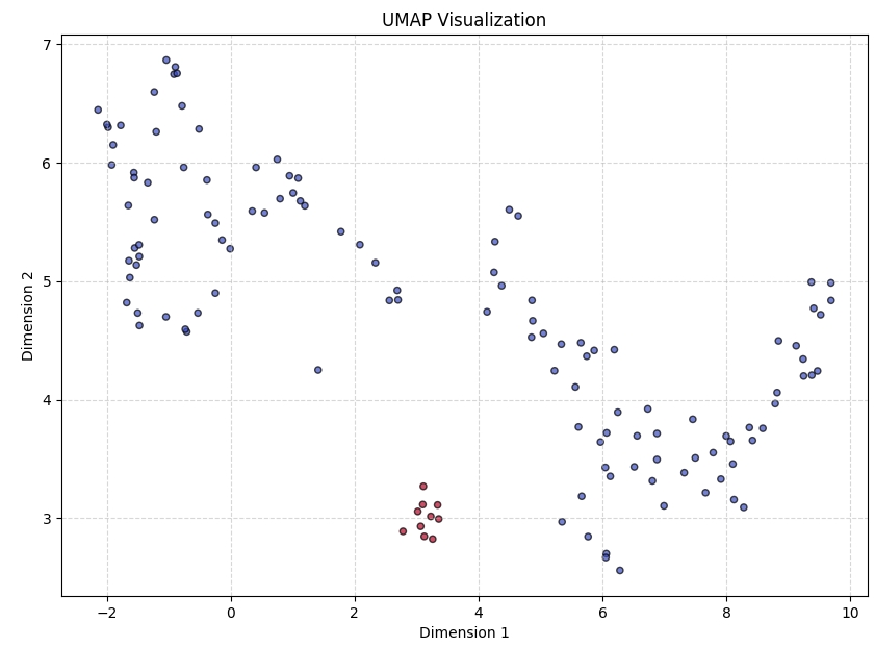
\includegraphics[width=1\linewidth]{Images/UMAP_n10.pdf}
    \caption{UMAP with $n_{neighbors} = 10$ and $min_{dist} = 0.1$.}
    \label{fig:umap_10}
\end{figure}

\begin{figure}[h] 
    \centering
    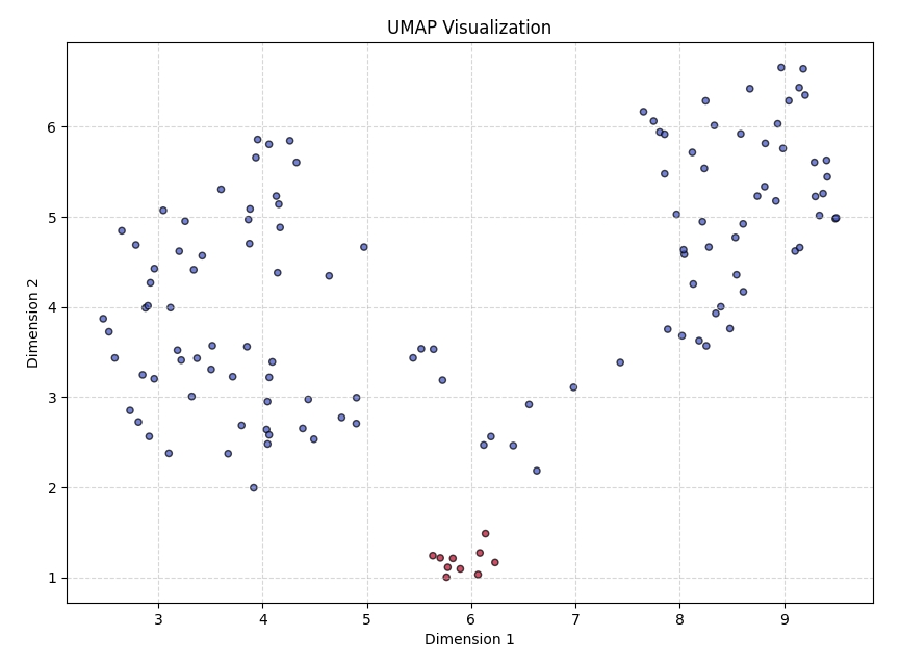
\includegraphics[width=1\linewidth]{Images/UMAP_n20.pdf}
    \caption{UMAP with $n_{neighbors} =20$ and $min_{dist} = 0.1$.}
    \label{fig:umap_20}
\end{figure}

\begin{figure}[h] 
    \centering
    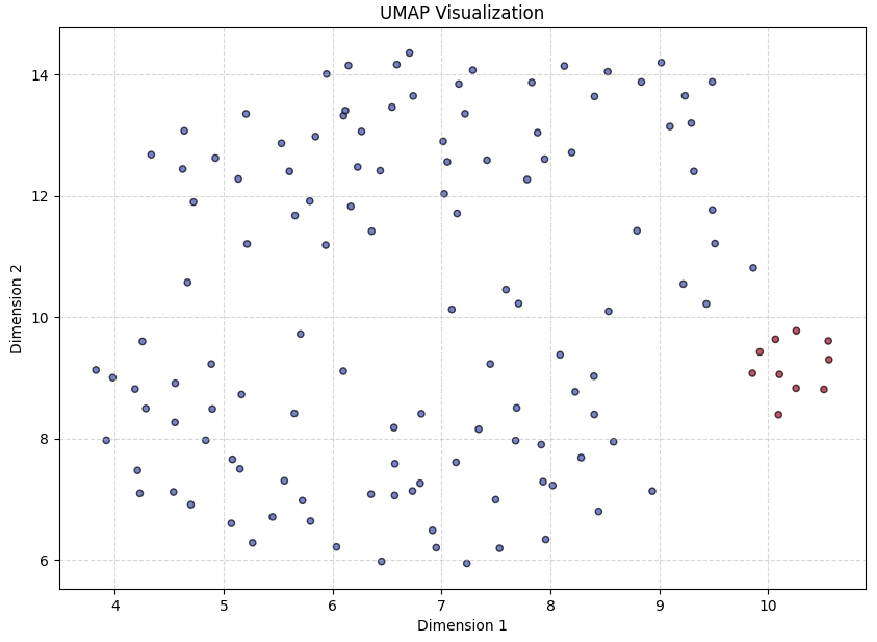
\includegraphics[width=1\linewidth]{Images/UMAP_d05.pdf}
    \caption{UMAP with $n_{neighbors} = 15$ and $min_{dist} = 0.5$.}
    \label{fig:umap_0.5}
\end{figure}

